%!TEX program = xelatex
\documentclass[UTF8,a4paper,zihao=-4,fontset=windows]{ctexart}

\usepackage[top=2.5cm,bottom=2.5cm,left=2.5cm,right=2.5cm]{geometry}
\usepackage{amsmath,amssymb,bm,mathtools}
\usepackage{booktabs,longtable,tabularx,array,multirow,makecell,threeparttable}
\usepackage{graphicx,subcaption,float,placeins}
\usepackage{xcolor}
\usepackage{enumitem}
\usepackage{setspace}
\usepackage{fancyhdr}
\usepackage{caption}
\usepackage{listings}
\usepackage{hyperref}
\usepackage{xurl}
\usepackage{etoolbox}
\usepackage{lastpage}

\setmainfont{Times New Roman}
\setmonofont{Cascadia Mono}
\setCJKmainfont[AutoFakeBold=2]{SimSun}
\setCJKsansfont[AutoFakeBold=2]{SimHei}

\definecolor{ink}{HTML}{20242A}
\definecolor{accent}{HTML}{276FBF}
\definecolor{muted}{HTML}{5F6B76}
\definecolor{linegray}{HTML}{B7C0C7}
\definecolor{codebg}{HTML}{F6F8FA}

\ctexset{
  section={format=\centering\heiti\zihao{4}\bfseries,beforeskip=12pt,afterskip=8pt},
  subsection={format=\heiti\zihao{-4}\bfseries,beforeskip=9pt,afterskip=4pt},
  subsubsection={format=\songti\zihao{-4}\bfseries,beforeskip=7pt,afterskip=3pt}
}

\setlength{\parindent}{2em}
\setlength{\parskip}{0pt}
\setlength{\footskip}{1.15cm}
\setlength{\emergencystretch}{2em}
\singlespacing
\setlist{nosep,leftmargin=2em}
\renewcommand{\arraystretch}{1.18}
\setlength{\tabcolsep}{4.5pt}

\pagestyle{fancy}
\fancyhf{}
\cfoot{\zihao{5}\thepage}
\renewcommand{\headrulewidth}{0pt}
\renewcommand{\footrulewidth}{0pt}

\DeclareCaptionFont{wuhao}{\zihao{5}\songti\color{black}}
\captionsetup{font=wuhao,labelfont=wuhao,labelsep=quad,justification=centering}
\captionsetup[figure]{position=bottom,skip=5pt}
\captionsetup[table]{position=top,skip=5pt}
\AtBeginEnvironment{tabular}{\zihao{5}\songti}
\AtBeginEnvironment{tabularx}{\zihao{5}\songti}
\AtBeginEnvironment{longtable}{\zihao{5}\songti}
\graphicspath{{../supporting_materials/figures/paper_final/}}

\newcommand{\unit}[1]{\,\mathrm{#1}}
\newcommand{\R}{\mathcal{R}}
\newcommand{\T}{\mathcal{T}}
\newcommand{\I}{\mathcal{I}}
\newcommand{\J}{\mathcal{J}}
\newcommand{\D}{\mathcal{D}}
\newcommand{\Ecal}{\mathcal{E}}
\newcommand{\E}{\mathbb{E}}
\newcommand{\indicator}{\mathbb{I}}

\lstdefinestyle{paperpython}{
  language=Python,
  basicstyle=\ttfamily\zihao{-5},
  keywordstyle=\color{accent},
  commentstyle=\color{muted},
  stringstyle=\color{ink},
  backgroundcolor=\color{codebg},
  frame=single,
  rulecolor=\color{linegray},
  numbers=left,
  numberstyle=\tiny\color{muted},
  breaklines=true,
  breakatwhitespace=false,
  showstringspaces=false,
  tabsize=4,
  columns=fullflexible,
  keepspaces=true,
  literate={Ⅰ}{{I}}1 {Ⅱ}{{II}}2 {Ⅲ}{{III}}3 {Ⅳ}{{IV}}2
}

\hypersetup{hidelinks,pdftitle={共享设备与医生约束下的超声预约联合优化},pdfauthor={},pdfsubject={数学建模竞赛论文},pdflang={zh-CN}}

\makeatletter
\patchcmd{\thebibliography}{\section*{\refname}}{}{}{}
\makeatother

\begin{document}
\songti\zihao{-4}\color{ink}
\pagenumbering{arabic}

\begin{center}
  \vspace*{0.10cm}
  {\heiti\zihao{3}\bfseries 共享设备与医生约束下的超声预约联合优化}\par
  \vspace{14pt}
  {\heiti\zihao{4}\bfseries 摘\quad 要}
\end{center}

超声预约不是单机排队问题：同一患者可能包含多个检查项目，项目对设备能力存在选择限制，检查过程还同时占用医生；空腹、憋尿、床旁检查和跨室转运又改变了可用时间窗。针对这些特点，本文以题目给出的住院、门诊、体检记录及22台设备资料为基础，建立“参数标定—统一任务表示—连续日历排程—留出期评价”的患者级联合模型。模型参数只由2019年3月1日至2024年3月31日训练期估计，2024年4月1日至2025年3月31日仅用于时间顺序检验；由于住院事件的最大截止期为48小时，只在留出边界前加2日预热，用于携入真正可跨边界的在制任务。

对于问题一，先以“患者编号+精确开单时刻”构造申请事件，去除打印、预约等非扫查项目，并按互斥优先级将服务项目归入11类。题目没有扫查起止时刻，故不把报告间隔解释为实测检查时长，而以题给时长区间的中点作为名义值、上界作为复杂病例值；单项目相邻报告间隔和医生日吞吐仅用于形成相对修正。训练期得到297\,656个住院、245\,614个门诊和239\,569个体检事件，形成42\,336个医生—项目完整调度时长估计，其中6\,416个组合具有直接间隔证据。设备能力以表1项目文本为直接证据来源，建立项目级严格匹配、类别回退和床旁明确三层证据；22台设备中床旁检查仅7号机可承担，是确定性唯一瓶颈。医生容量则由表6训练日首末活动时段重构为星期—5分钟槽并发上限，主情景为5至20人，而非把每日医生总数复制到每个机房。

对于问题二，将每位住院患者的全部服务项目作为一个不可拆分完成目标，在5分钟离散连续日历上同时决定患者顺序、项目内部顺序、开始时刻与机房。模型约束包括设备互斥、医生共享并发、项目—设备兼容、患者自身不重叠、48小时截止、空腹10时前完成、憋尿准备、床旁7号机、同室优先及跨室至少10分钟转运。采用“共同机房优先—多候选项目序列—最早可行时隙”的构造算法，并分别比较共享先到先服务、最小松弛度保护和联合稀缺度策略。

对于问题三，把门诊和体检的历史报告日期作为回顾性计划日压力场景，不读取历史报告时刻、机房和医生派单；释放时刻不早于真实开单，三类患者在同一个年度日历中竞争相同房间与医生容量。主情景将留出期中按整数事件最接近5\%的8\,341个事件设为复杂病例，其项目采用时长上界。留出期共有70\,771个住院事件和96\,046个门诊/体检事件。题目未给出“满足门诊、体检需求”的数值阈值，故以共享FCFS的计划日服务率作为不劣基线，再按住院48小时率选择主方案。资源可行FCFS完成45\,260个住院事件，48小时率63.95\%，并完成57\,341个门诊/体检计划日事件，完成率59.70\%；联合稀缺度把背景率提高到61.61\%，却使住院率降至63.31\%，因此只作为帕累托备选。独立程序重构151\,020条排程任务，对房间重叠、医生超容量、患者冲突、兼容、转运、准备约束、时长和结果聚合等18项检查，违规数均为0。敏感性分析表明，医生容量降至训练日下四分位时住院率下降1.99个百分点；仅保留严格设备证据会使背景完成率下降10.03个百分点，说明上线前必须由超声科确认回退项目清单。

本文最终给出可直接执行的患者—项目—时段—机房推荐表。由于数据缺少真实预约时刻、扫查结束、报告提交时刻、未来医生身份和项目资质矩阵，本文把“排程中最后一个项目结束”作为报告完成代理，结果应理解为预约决策方案与能力压力评估，而不是对临床报告时效的因果结论。

\vspace{7pt}
\noindent\textbf{关键词：}超声预约；患者级排程；共享资源；48小时完成率；设备兼容；敏感性分析

\clearpage
\section{问题重述}

\subsection{问题背景}

某医院超声科同时接收住院、门诊和体检三类检查申请。一次申请可能包含多个项目，各项目在检查时长、准备条件和可用设备上存在差异；22台设备具有明确的专项分工，医生又在不同设备之间共享。任一时刻，一台设备只能承担一项检查，同一患者的多个项目也不能并行执行。住院患者还受到开单后48小时完成全部项目的时限约束，门诊与体检需求则集中占用计划日内的服务容量。医疗预约研究通常需要同时处理等待、容量和服务水平\cite{gupta2008,ahmadi2017}，分时预约和检查资源协同也是改善候检秩序的重要手段\cite{nhc2020,chenjuan2023}，因此需要在设备能力、人员容量与患者完整流程之间进行统一配置。

\subsection{问题重述}

根据题目给出的历史检查记录、设备项目说明和医生信息，需要分析超声需求与资源状态，并针对纯住院场景及三类患者共享资源场景制定预约优化方案。具体需要完成以下三个问题：

（1）分析住院、门诊和体检需求随日期、科室与项目的变化，识别平峰、高峰及压力状态，估计项目工时和医生并发能力，并据此给出设备开放、专项资源保留和预约分流原则。

（2）仅考虑住院患者，在48小时内完整完成全部检查的口径下，确定患者主序、项目次序、检查时刻和所用设备，使完成事件数尽可能多，并输出患者级预约与检查顺序。

（3）在问题二的资源约束基础上加入门诊和体检患者，建立三类患者联合调度模型，刻画背景服务率与住院48小时完成率之间的交换关系，选择可实施的折中方案并检验其稳定性。

\section{问题分析}

\subsection{字段语义与数据口径}

住院、门诊、体检三张明细均以项目行为基本单位，同一患者同一开单时刻可以出现多行。若直接把明细行视为患者，会重复计算多项目申请；若只按患者编号聚合，又会把同一患者不同时期的多次申请合并。因此定义申请事件键
\begin{equation}
  e=(s,p,a),
\end{equation}
其中$s$为来源，$p$为患者编号，$a$为精确开单时刻；患者编号缺失时以来源行号构造只在该表内唯一的代理键。对同一事件内完全相同的服务项目去重，而不同项目全部保留。打印、预约和图文报告等不占用超声扫查设备的记录被标记为非服务项，不进入工作量。

时间字段分为到达与完成两类。住院释放时刻取开单时刻$a_e$，截止时刻为$d_e=a_e+48\unit{h}$。门诊和体检缺少真实预约日期，本文只在回顾性评价中使用报告日期构造计划日$g_e$；其日内窗口为上午$[8{:}00,12{:}00]$和下午$[13{:}00,17{:}00]$。历史报告的具体时分、历史机房和历史医生不进入决策。官方质量指标强调以申请单为分母评价完成情况\cite{nhc2022}，但附件又缺少独立的报告提交时刻，因此本文将排程中最后一个项目结束时刻作为“完成检查并可进入报告环节”的代理，全文不把它表述为真实报告提交时间。

\begin{table}[H]
  \centering
  \caption{统一连续模拟与留出期评价规模}
  \label{tab:data-scope}
  \begin{tabular}{lrrr}
\toprule
患者来源 & 连续模拟事件数 & 项目任务数 & 留出期评价事件数 \\
\midrule
住院 & 71,029 & 141,429 & 70,771 \\
门诊 & 55,512 & 69,756 & 55,226 \\
体检 & 40,820 & 117,701 & 40,820 \\
\midrule
合计 & 167,361 & 328,886 & 166,817 \\
\bottomrule
\end{tabular}

\end{table}

连续模拟规模见表\ref{tab:data-scope}。其中住院事件在2日预热期和一年留出期均保留精确开单时刻；门诊与体检只使用计划日压力，不使用历史派单结果。这一处理使问题三能够使用三类患者的真实项目组合和日需求，同时避免把不可获得的未来机房、医生当作模型输入。

\subsection{项目归类与资源标记}

项目归类采用互斥优先级词典。首先识别非服务项；随后依次识别产科III/IV级、产科I/II级、心脏、介入/定位、血管、腔内、腹部/胃肠、浅表器官、儿科专项和一般其他。优先级解决关键词重叠，例如“心脏造影”先被识别为心脏项目，不因包含“造影”而误入介入类别。每个项目族的时长边界直接依据题给区间，并保留项目原名用于设备匹配，不以类别名替代项目名。

题目中的检查准备要求转换为三个事件级标记：包含“空腹”的项目必须在10时前完成；包含“充盈膀胱”等词的事件在主情景中以开单后60分钟作为准备完成时刻，另以45和90分钟作敏感性；若门诊/体检在计划日开班前已满足提前量，则从工作块起点即可排入；明确“床旁”的检查只允许7号床边B超机。若一个事件同时包含多个标记，所有相应约束共同生效。

\subsection{时间边界和中文名称泄漏控制}

用于建模的项目目录只统计训练期出现的项目名称。留出期项目在调度输入中按训练期确定的归类规则处理；若新名称无法获得项目级设备证据，才进入已标注的类别回退。另输出全期项目目录只用于检查名称漂移，不参与留出期派位。医生效率和报告间隔同样只使用2024年3月31日以前的报告记录，避免利用留出期完成时刻修正未来调度速度。

\subsection{需求变化与高峰特征}

图\ref{fig:monthly-demand}给出三类患者月度日均开单量。住院需求总体平稳上升；门诊呈较强年度和节假日波动；体检最不稳定，在团检月份形成尖峰。因而用全年平均值配置日容量会同时低估体检高峰和住院周一压力。本文在问题一中分别计算来源内日中位数、90\%分位和95\%分位，并保留星期结构，不把“高峰”定义为简单事件数最多的若干天。

\begin{figure}[H]
  \centering
  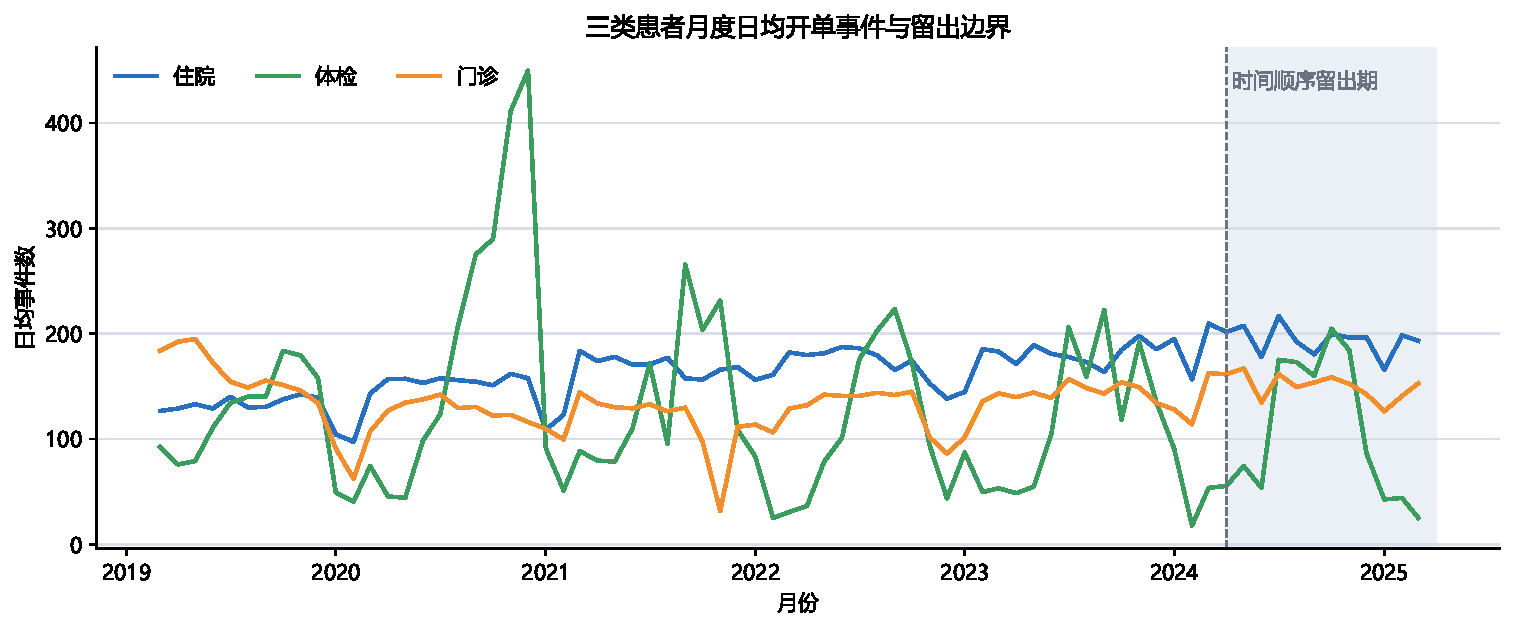
\includegraphics[width=\textwidth]{fig01_monthly_demand.pdf}
  \caption{三类患者月度日均开单量及时间顺序留出边界}
  \label{fig:monthly-demand}
\end{figure}

训练期科室需求见表\ref{tab:department}. 住院需求分散于87个可识别科室，前6科室占35.45\%；门诊需求集中度更高，前6科室占62.95\%；体检记录只有一个科室编码，不能据此推断其临床科室组成。科室字段缺失的事件数量很少，但模型仍在结果中保留“缺失”类别，不使用众数强行填补。

\begin{table}[H]
  \centering
  \caption{训练期科室需求集中度}
  \label{tab:department}
  \begin{tabular}{lrrrr}
\toprule
来源 & 训练期事件数 & 可识别科室数 & 前6科室占比 & 前12科室占比 \\
\midrule
住院 & 297,656 & 87 & 35.45\% & 56.72\% \\
门诊 & 245,614 & 133 & 62.95\% & 81.33\% \\
体检 & 239,569 & 1 & 100.00\% & 100.00\% \\
\bottomrule
\end{tabular}

\end{table}

\subsection{数据能够支持与不能支持的结论}

数据能够支持：事件到达规模、项目组合、题给时长边界、项目文本对应的设备能力、历史医生活动时段以及留出期回顾性压力测试。数据不能直接支持：真实扫查时长、报告撰写时长、未来医生身份与项目资质、真实预约时刻、未完成患者的真实后续处置。过程挖掘中的相邻时间戳不自动等于活动持续时间\cite{vda2011}，影像报告时间的测量也必须区分图像采集、阅片和报告环节\cite{sexauer2022}。因此，本文所有“时长估计”均称为调度占用参数，所有“完成率”均注明代理边界。

\section{模型假设}

1、假设同一患者编号与同一精确开单时刻对应一次完整检查申请；医嘱字段中以“][”连接的内容表示分别计费的项目，应拆为同一事件下的多个任务。该假设直接对应源系统字段结构。

2、假设题目给出的项目时长区间能够代表标准检查工时；名义场景取区间中点，题目所述5\%复杂检查取区间上界。由于附件没有复杂病例标签，主结果用固定随机种子抽取，并用5个额外种子检验。

3、假设工作模板为每日08:00--12:00和13:00--17:00，检查不得跨越午休或日界。该模板由训练期医生首末活动记录重构，是标准日班压力场景，不解释为医院正式排班表。

4、假设任一项目同时占用一台兼容设备和一名医生；设备独占，医生以星期—5分钟槽总并发容量表示。题面33名未来医生与历史ID无法一一映射，因此不虚构实名医生专项资质矩阵。

5、假设项目—设备兼容只由题目表1的项目文本确定；允许直接名称、明确同义或包含关系以及题面明确的广义项目描述，复合项目取组成项目的同设备交集。无法从表1确认的项目不进入候选设备集合。

6、假设床旁表示检查地点而非项目能力。床旁任务只有在项目本身与7号机能力相容时才可使用7号机，床旁标记不能覆盖心脏、血管、产科、介入等专项要求。

7、假设腹部、胃肠和肠系膜等空腹项目须在10:00前完成；憋尿项目在开单后至少准备60分钟。项目准备类型对应公开超声检查流程中的空腹与充盈膀胱要求\cite{hrhospital2025}，具体60分钟提前量由敏感性界定。准备约束按项目粒度施加，事件级统一准备作为对照情景。

8、假设同一患者的两个项目不能重叠；跨设备相邻项目至少留10分钟转运，同设备连续项目不额外计转运。5分钟和15分钟边界另行检验。

9、假设住院事件在开单后48小时内全部项目完成才计为达标；未排入、项目缺失或任一项目越过截止均记为未完成，分母不因能力缺失而减少。

10、假设门诊、体检报告日期可作为回顾性计划日压力代理，但不能还原真实预约日期；其最后项目在计划日17:00前结束记为计划日完成。本文据此讨论服务水平，不声称复原历史调度。

11、假设最后一个排程项目的结束时刻是报告完成的乐观代理。附件没有扫查结束、书写和提交时刻，故模型结果用于预约与容量评估，不能解释为真实报告时效的因果改善。

12、假设训练期结束于2024年3月31日，留出期从2024年4月1日至2025年3月31日。阈值、项目目录、医生容量和稀缺权重只读训练期；留出期仅用于评价，不反向调参。

\section{符号说明}

\begin{table}[H]
\centering
\caption{主要集合、参数与变量}
\label{tab:symbols}
\begin{tabularx}{\textwidth}{l X}
\toprule
符号 & 含义 \\
\midrule
$e\in\Ecal$ & 患者申请事件，含来源、患者、释放时刻和截止时刻 \\
$j\in\J_e$ & 事件$e$的服务项目；$n_e=|\J_e|$ \\
$r\in\R$ & 超声设备或对应检查房间，$|\R|=22$ \\
$t\in\T$ & 5分钟离散时隙；每天上午、下午各48个 \\
$q_e\in\{I,O,P\}$ & 事件来源：住院、门诊、体检 \\
$a_e,d_e$ & 事件释放时刻与截止时刻 \\
$p_{ej}^{(0)},p_{ej}^{(1)}$ & 项目名义时长和特殊病例上界时长（时隙数） \\
$z_e$ & 特殊病例标记，$\sum_e z_e/|\Ecal|=5\%$ \\
$\R_{ej}^{S},\R_{ej}^{F}$ & 项目的严格兼容设备集合与类别回退设备集合 \\
$\R_{ej}$ & 主情景可用设备集合；床旁项目固定为$\{7\}$ \\
$c_{wt}$ & 星期$w$、日内时隙$t$的医生并发容量 \\
$b_{ej},f_{ej},u_{ej}$ & 床旁、空腹、憋尿标记 \\
$\tau$ & 相邻项目跨室转运时长，主情景为10分钟 \\
$x_{ejrt}$ & 项目$(e,j)$是否在设备$r$、时隙$t$开始 \\
$y_e$ & 事件$e$是否全部项目在截止前完成 \\
$C_e,S_e$ & 事件完成时刻与首个项目开始时刻 \\
$L_r(t)$ & 时刻$t$前设备$r$的累计占用时隙数 \\
$\kappa_r$ & 设备$r$的需求稀缺度权重 \\
\bottomrule
\end{tabularx}
\end{table}

为避免与自然常数混淆，正文用$e$表示一个具体事件，用$\Ecal$表示事件集合；集合上标$S$和$F$分别表示严格证据与回退证据。完成率均按事件计算而非项目行计算：只有$n_e$个服务项目全部排入且最后完成时刻不晚于$d_e$，才有$y_e=1$。

\section{模型的建立与求解}

三个子问共用同一个患者事件、项目任务、设备能力和医生时隙容量内核。问题一估计需求与资源参数；问题二建立住院患者级排程；问题三只在共享日历中加入门诊和体检计划日约束，不另造一套不相容的容量模型。全年整数模型的变量规模过大，因而本文用整数规划明确数学可行域，用共享同一约束的确定性构造算法完成全年求解。
\subsection{问题一：需求、时长与资源配置模型}

\subsubsection{需求预测与峰平判定}

对来源$s$、日期$d$，记开单事件数为$N_{sd}$。为检验星期与趋势结构，比较三个不使用留出期信息的基准模型：7日季节朴素、最近8周同星期中位数和日历趋势岭回归。后者写为
\begin{equation}
  \widehat N_{sd}=\beta_0+\beta_1 t_d+\sum_{w=1}^{6}\gamma_w I(w_d=w)
  +\sum_{m=2}^{12}\eta_m I(m_d=m)+\rho_1\sin\frac{2\pi t_d}{365.25}
  +\rho_2\cos\frac{2\pi t_d}{365.25}.
\end{equation}
岭参数只在训练期设计矩阵上确定。采用
\begin{equation}
 \mathrm{WAPE}=\frac{\sum_d|N_{sd}-\widehat N_{sd}|}{\sum_dN_{sd}}
\end{equation}
作为主评价，因为体检低需求日会使逐日百分比误差不稳定。留出期结果表明：住院和门诊开单量均由最近8周同星期中位数取得最低WAPE，分别为16.04\%和14.04\%；体检开单量由日历趋势模型取得最低WAPE，但仍为69.83\%，说明团检尖峰不能靠常规日历变量充分预测。三类合计开单量的最低WAPE为24.92\%。医院日需求预测中显式建模星期结构并滚动验证是必要步骤\cite{luo2017,lin2019}，但体检业务还需要接入未来团检计划，不能只依赖历史时间序列。

对留出期每日需求分布，以中位数附近$[Q_{0.45},Q_{0.55}]$定义平峰，以$Q_{0.90}$定义高峰，以$Q_{0.95}$定义压力日。住院开单日平峰为197人，高峰阈值283人；门诊分别为156和198人；体检因团检尖峰，平峰48人而$Q_{0.90}$达到308.2人。故设备配置采用“固定能力底座+高峰弹性块”，而不是按体检全年均值永久占用机房。

\subsubsection{服务时长的分层估计}

设项目$j$属于类别$k(j)$，题给时长区间为$[l_k,u_k]$，名义时长
\begin{equation}
  p_j^{(0)}=5\left\lceil\frac{(l_k+u_k)/2}{5}\right\rceil,
  \qquad
  p_j^{(1)}=5\left\lceil\frac{u_k}{5}\right\rceil.
\end{equation}
5\%特殊事件使用$p_j^{(1)}$，其余使用$p_j^{(0)}$。各项目族参数见表\ref{tab:duration}。心脏、产科III/IV级的绝对占用显著高于一般项目，是高峰配置中必须保护的长任务。

同一申请含多个项目时，主排程按项目逐项累计上述时长；在同一兼容机房连续完成可以省去转运，但不把不同项目视为同时扫描。训练期另以0.8、0.9和1.0三种合并系数检查需求量口径，本文不把缺少现场证据的节约比例写入患者级可行域。

\begin{table}[H]
  \centering
  \caption{项目族调度时长及训练期间隔证据}
  \label{tab:duration}
  \begin{tabular}{lrrrr}
\toprule
项目族 & 下界/min & 名义/min & 上界/min & 训练期代理样本数 \\
\midrule
产科III/IV级 & 30 & 35 & 40 & 13,451 \\
产科I/II级 & 15 & 17.5 & 20 & 20,095 \\
心脏 & 10 & 12.5 & 15 & 141,017 \\
介入/定位 & 5 & 7.5 & 10 & 6,782 \\
血管 & 5 & 7.5 & 10 & 59,006 \\
经阴道/腔内 & 5 & 7.5 & 10 & 21,244 \\
泌尿/经腹妇科 & 5 & 7.5 & 10 & 75,137 \\
腹部/胃肠 & 5 & 7.5 & 10 & 99,719 \\
浅表器官 & 5 & 7.5 & 10 & 67,825 \\
儿科专项 & 5 & 7.5 & 10 & 3,950 \\
一般其他 & 5 & 7.5 & 10 & 3,400 \\
\bottomrule
\end{tabular}

\end{table}

为描述医生异质性，先选取同一医生、同一天的单项目事件，计算相邻报告间隔$g_n$，仅保留$0<g_n\leq60$分钟。对医生$i$，由有效工作日吞吐量得到对数相对因子$h_i$，再作经验贝叶斯收缩：
\begin{equation}
  \widetilde h_i=\omega_i h_i+(1-\omega_i)\mu_h,
  \qquad
  \omega_i=\frac{m_i}{m_i+\lambda},
\end{equation}
其中$m_i$为有效工作日数，$\mu_h$为总体对数吞吐均值。医生—项目组合的调度时长取直接间隔中位数与题给名义时长经医生因子修正后的收缩组合，并截断在$[l_k,u_k]$内。该方法形成42\,336个完整组合、6\,416个直接证据组合。由于相邻报告间隔包含非扫查活动，$\widetilde h_i$只用于相对速度与能力分析，患者级主排程仍采用题给绝对时长，以免把代理噪声固化为硬约束。基于检查类别预测超声检查时长具有现实依据\cite{lai2025}，但本文对字段缺失作了更保守的解释。

\subsubsection{项目—设备能力证据}

设备能力从表1的检查项目文本逐项建立。对项目名称$q$和设备$r$定义三级匹配：
\begin{equation}
  A_{qr}=\begin{cases}
  2,&\text{项目名称精确、包含或语义核心匹配；}\\
  1,&\text{无项目级证据但项目族有具体能力证据；}\\
  3,&\text{文本明确为床旁且$r=7$；}\\
  0,&\text{否则。}
  \end{cases}
\end{equation}
主情景允许$A_{qr}\geq1$，同时记录$A_{qr}=1$的回退任务；严格敏感性只允许$A_{qr}\in\{2,3\}$。宽泛描述如“常规项目”不能单独建立某个项目族的硬能力。图\ref{fig:coverage}显示，住院、门诊任务的严格或床旁证据分别达到98.2\%和91.2\%，体检只有69.4\%，其余30.6\%依赖类别回退。这一差异决定了问题三不能只报告总兼容率。

\begin{figure}[H]
  \centering
  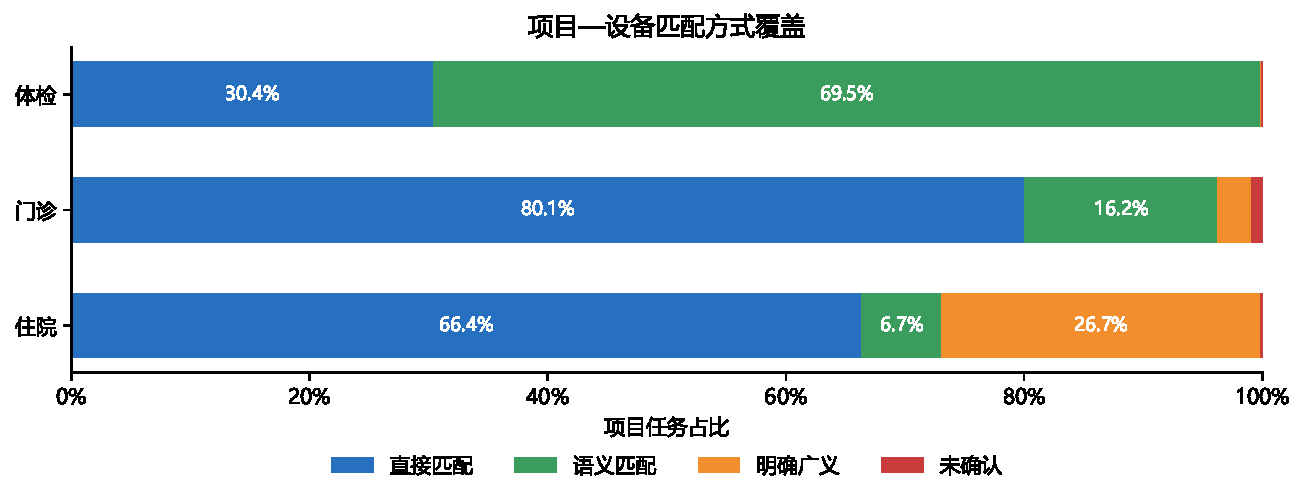
\includegraphics[width=0.92\textwidth]{fig03_capability_coverage.pdf}
  \caption{三类患者项目—设备兼容证据覆盖}
  \label{fig:coverage}
\end{figure}

关键资源见表\ref{tab:capability}. 床旁仅7号机可执行；产科III/IV级集中于64、43、65号三台设备；儿科专项仅45、44号两台。心脏、血管等项目虽有较多可用设备，但长时长和高需求仍会形成负荷瓶颈。

\begin{table}[H]
  \centering
  \caption{关键资源的设备覆盖与结构判断}
  \label{tab:capability}
  \begin{tabularx}{\textwidth}{l r X l}
\toprule
关键资源 & 可用设备数 & 设备编号 & 结构判断 \\
\midrule
床旁 & 1 & 7 & 唯一瓶颈 \\
心脏 & 5 & 73|113|48|45|49 & 多房间 \\
血管 & 12 & 40|69|72|71|41|42|46|47|44|74|75|77 & 多房间 \\
III/IV产科 & 3 & 64|43|65 & 少数房间 \\
I/II产科 & 13 & 40|41|42|46|47|44|64|43|65|160|74|75|77 & 多房间 \\
儿科专项 & 2 & 45|44 & 少数房间 \\
介入/定位 & 15 & 40|69|72|41|42|46|47|44|64|43|65|160|74|75|77 & 多房间 \\
\bottomrule
\end{tabularx}

\end{table}

\subsubsection{医生共享时隙容量}

表6提供医生每日项目数及首末活动时刻。对训练日$d$和5分钟槽$t$，若$t$位于医生$i$重构活动区间内，则$I_{idt}=1$。星期$w$的主容量和偏紧容量分别为
\begin{equation}
  c^{(0)}_{wt}=\min\left\{22,\operatorname{Med}_{d:\,w(d)=w}\sum_iI_{idt}\right\},
  \quad
  c^{(L)}_{wt}=\min\left\{22,Q_{0.25,d:\,w(d)=w}\sum_iI_{idt}\right\}.
\end{equation}
首活动在7--9时之间归整为8时开班，12:30--14时归整为13时开班；末活动在11--12:30归整为12时，在16--19时归整为17时，其他情况保留观察区间并向前扩10分钟。该规则只修复报告时间代理对班次边界的轻微偏移，不把单个医生复制成全天可用。

\begin{figure}[H]
  \centering
  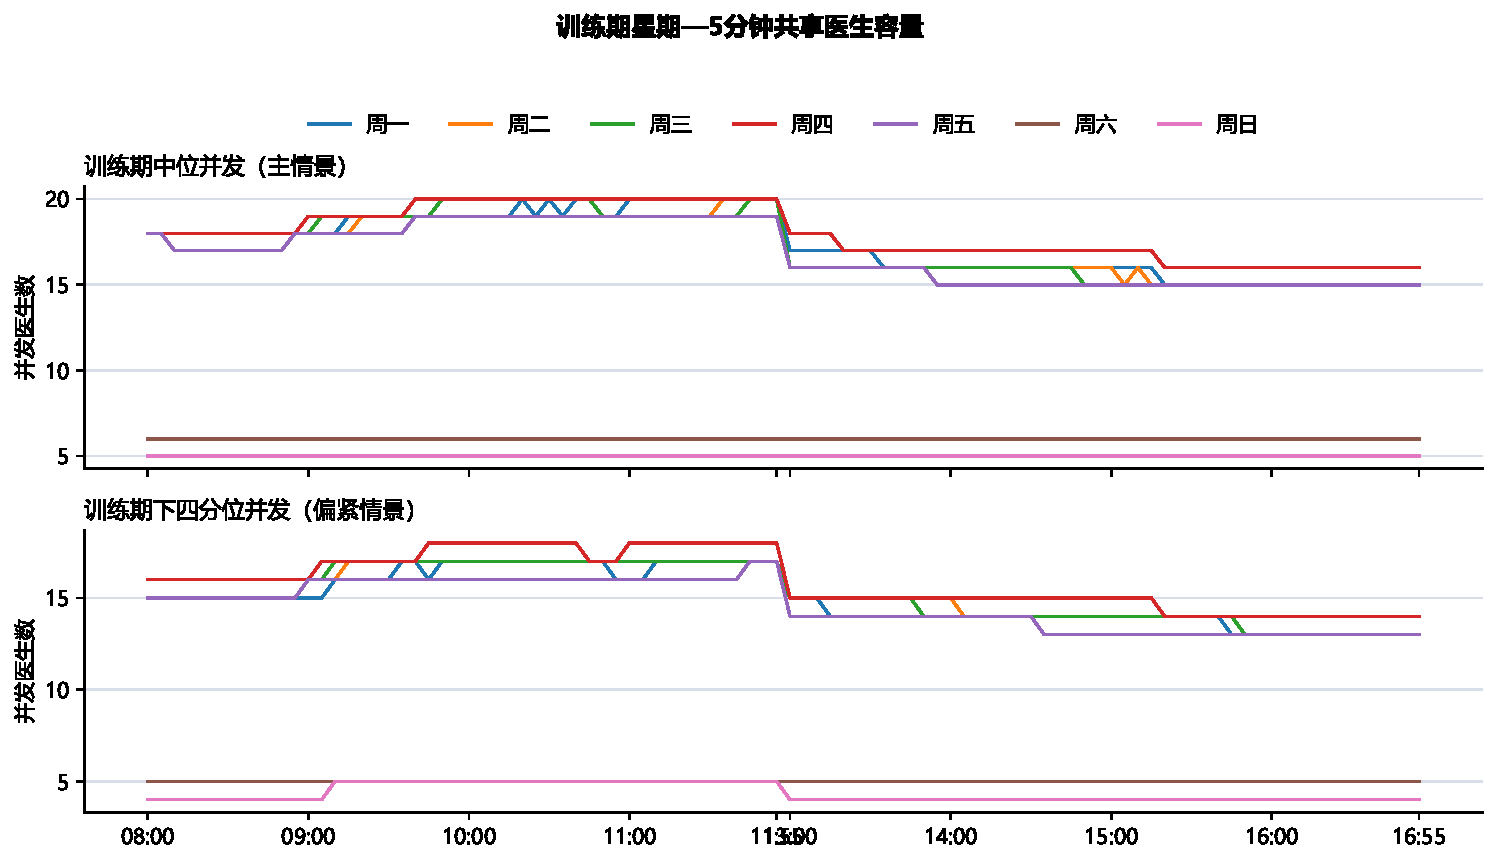
\includegraphics[width=\textwidth]{fig02_doctor_capacity.pdf}
  \caption{训练期重构的星期—时隙医生共享容量}
  \label{fig:doctor-capacity}
\end{figure}

\begin{table}[H]
  \centering
  \caption{各星期医生并发容量范围}
  \label{tab:doctor-capacity}
  \begin{tabular}{lrrrrrr}
\toprule
 & \multicolumn{3}{c}{主情景} & \multicolumn{3}{c}{偏紧情景} \\
\cmidrule(lr){2-4}\cmidrule(lr){5-7}
星期 & 最小 & 中位 & 最大 & 最小 & 中位 & 最大 \\
\midrule
周一 & 15 & 17.5 & 20 & 13 & 15 & 17 \\
周二 & 15 & 17 & 20 & 14 & 15.5 & 17 \\
周三 & 15 & 17 & 20 & 13 & 15.5 & 17 \\
周四 & 16 & 18 & 20 & 14 & 15.5 & 18 \\
周五 & 15 & 16.5 & 19 & 13 & 14.5 & 17 \\
周六 & 6 & 6 & 6 & 5 & 5 & 5 \\
周日 & 5 & 5 & 5 & 4 & 4 & 5 \\
\bottomrule
\end{tabular}

\end{table}

工作日主容量为15--20人，周六为6人，周日为5人；实际可同时运行的设备数取设备数22与$c_{wt}$的较小值。图\ref{fig:doctor-capacity}表明午后容量普遍略低，周末更明显。医生下四分位情景将用于检验人力不足风险。

\subsubsection{峰平配置方案}

综合需求、能力和医生容量，提出以下配置原则。

\begin{enumerate}
  \item 7号机全天保留床旁任务，非床旁项目只有在确定不会挤占床旁窗口时才可回填；这是唯一确定性硬瓶颈。
  \item 64、43、65号设备形成产科III/IV级保护池；45、44号形成儿科保护池。其余兼容机房按项目稀缺度分配，灵活项目优先使用覆盖面较广且当前负荷较低的设备。
  \item 平峰按训练期中位需求开放固定能力底座；高峰不固定新增某台“万能机”，而是在上午空腹块和下午非空腹块分别释放弹性时隙。体检团检高峰需提前导入团检名单，单独预留成块容量。
  \item 5\%特殊病例不另设固定机房，而在每个工作块保留与上界时长差对应的缓冲。医生并发低于设备数时，先补医生班次而不是继续开放设备。
\end{enumerate}

表\ref{tab:peak-flat-plan}把上述原则落实为22台现有设备的运行配置。这里的“开放”表示允许排程占用，并不等于临时购置设备；任一时刻真正可并行工作的台数仍受$c_{wt}$限制。

\begin{table}[H]
  \centering
  \caption{22台现有设备的峰平运行配置}
  \label{tab:peak-flat-plan}
  \begin{tabularx}{\textwidth}{p{0.19\textwidth} c X X}
    \toprule
    资源池 & 台数 & 平峰配置 & 高峰/压力配置 \\
    \midrule
    床旁7号机 & 1 & 床旁任务保护，确认无待服务床旁任务时才回填 & 保持床旁专用，不以普通任务填满 \\
    产科III/IV级（64、43、65） & 3 & 保留专项能力，按实际产科项目启用 & 三台均进入专项候选，空余槽才承接兼容任务 \\
    儿科专项（45、44） & 2 & 保留儿科能力，空余槽可按证据回填 & 两台均保护儿科窗口，避免一般项目提前占用 \\
    其余兼容设备 & 16 & 按$Q_{0.45}$--$Q_{0.55}$工作量滚动开放 & 按$Q_{0.90}$需求和已知团检名单释放成块时隙；$Q_{0.95}$压力日先增医生班次 \\
    \bottomrule
  \end{tabularx}
\end{table}

该方案既回答了“哪些机器配置哪些项目”，又保留了患者级模型根据当日项目组合动态选择具体机房的空间；固定配置负责保护稀缺能力，滚动排程负责利用可替代能力。

\subsection{问题二：住院患者48小时排程模型}

\subsubsection{患者级离散时间模型}

对住院事件$e$，项目$j\in\J_e$需要$p_{ej}$个5分钟时隙，可用设备集合为$\R_{ej}$。若项目在设备$r$、时隙$t$开始，令$x_{ejrt}=1$。每个项目至多开始一次：
\begin{equation}
  \sum_{r\in\R_{ej}}\sum_{t\in\T_{ej}}x_{ejrt}\leq1,
  \qquad e\in\Ecal,\;j\in\J_e,
  \label{eq:once}
\end{equation}
其中$\T_{ej}$已剔除释放前、截止后、跨午休和跨日的开始时隙。事件是否全部完成由
\begin{equation}
  n_e y_e\leq\sum_{j\in\J_e}\sum_{r,t}x_{ejrt},
  \qquad y_e\in\{0,1\}
  \label{eq:complete}
\end{equation}
连接；因此多项目患者缺少任一项目时$y_e=0$。

设备互斥约束为
\begin{equation}
  \sum_{e,j}\sum_{t':\,t'\leq t<t'+p_{ej}}x_{ejrt'}\leq1,
  \qquad r\in\R,\;t\in\T.
  \label{eq:room}
\end{equation}
医生是所有机房共享的并发资源：
\begin{equation}
  \sum_{e,j,r}\sum_{t':\,t'\leq t<t'+p_{ej}}x_{ejrt'}\leq c_{w(t),s(t)},
  \qquad t\in\T,
  \label{eq:doctor}
\end{equation}
其中$w(t)$为星期，$s(t)$为日内槽。式\eqref{eq:doctor}防止把同一批医生分别复制给22台设备。

\subsubsection{患者内部顺序与准备约束}

同一患者的项目必须串行。若项目$j$在$j'$之前，记$o_{ejj'}=1$，则
\begin{align}
  S_{ej'}&\geq S_{ej}+p_{ej}+\tau v_{ejj'}-M(1-o_{ejj'}),\\
  S_{ej}&\geq S_{ej'}+p_{ej'}+\tau v_{ej'j}-Mo_{ejj'},
  \label{eq:precedence}
\end{align}
其中$v_{ejj'}=1$表示相邻项目不在同一设备，$\tau=2$个时隙。对$n_e>2$的事件，精确整数模型还需引入序位变量消除子环。大规模求解中直接构造一个完整项目序列，天然满足式\eqref{eq:precedence}。

空腹项目的完成时刻满足
\begin{equation}
  S_{ej}+p_{ej}\leq 10{:}00,
  \qquad f_{ej}=1.
\end{equation}
憋尿事件的有效释放时刻为$a'_e=a_e+\delta_e$，主情景$\delta_e=60$分钟；床旁项目令$\R_{ej}=\{7\}$。其他项目不得因为患者包含床旁标记而自动绕过项目兼容，每个项目仍按自身能力集合安排。

\subsubsection{目标函数}

问题二的首要目标是最大化48小时内完成全部项目的患者数：
\begin{equation}
  \max Z_1=\sum_{e\in\Ecal_I}y_e.
  \label{eq:p2-primary}
\end{equation}
在$Z_1$固定后，依次最小化首检等待、跨室次数和设备负荷不均衡：
\begin{align}
  \min Z_2&=\sum_{e:y_e=1}(S_e-a'_e),\\
  \min Z_3&=\sum_{e,j,j'}v_{ejj'},\\
  \min Z_4&=\sum_{r\in\R}\left|L_r-\frac{1}{|\R|}\sum_{r'}L_{r'}\right|.
\end{align}
采用词典序而非$Z_1-\alpha Z_2-\beta Z_3$，是为了避免任意权重让若干分钟等待抵消一个患者的48小时成功。带患者优先级和时限保证的动态诊断资源调度也常采用服务水平优先的结构\cite{patrick2008,bauerhenne2026}。

\subsubsection{大规模构造算法}

全年事件和项目数使全时域MILP规模过大。本文保留上述整数模型作为结构定义，再采用与其共享可行域的确定性构造算法。

对每个事件，先计算项目的可用设备数$|\R_{ej}|$和工作量$p_{ej}$，形成四个候选项目序列：空腹优先且稀缺优先、空腹优先且长任务优先、纯稀缺优先、原始项目序。若所有项目存在共同设备，先在累计负荷最低的三个共同设备中依次寻找完整方案；共同设备快捷搜索不可行时，逐个候选序列在\textbf{全部}兼容设备中寻找最早可行时隙，并在换室处插入10分钟转运。因此“三个”只是全年构造算法的同室优先搜索宽度，不是现实中的设备数量限制，也不从可行集合中删除其他设备。只有事件全部项目都找到时才提交占用；任一项目失败则释放本次试排的全部槽，不产生“半个患者已排”的状态。

设备选择不仅看当前负荷，还定义背景需求稀缺权重
\begin{equation}
  \kappa_r=\sum_{e,j:\,r\in\R_{ej}}\frac{p_{ej}}{|\R_{ej}|}.
\end{equation}
式中求和只使用2019年3月1日至2024年3月31日训练期形成的项目目录与时长，不读取留出期项目构成。在同一最早时刻有多台设备可行时，先保留患者上一个房间，再选累计负荷低、$\kappa_r$较小的设备；这使灵活任务尽量不占用稀缺设备。

\subsubsection{策略定义}

比较三种策略：

\begin{enumerate}
  \item \textbf{共享FCFS：}门诊/体检按计划日和释放顺序排入，住院按释放时刻排序；设备先取最早可行时刻，同刻再按编号选择。
  \item \textbf{松弛度保护：}背景部分与共享FCFS相同；住院按$\sigma_e=d_e-p_e$排序，其中$p_e=\sum_jp_{ej}$，优先处理剩余余量小的多项目患者。
  \item \textbf{联合稀缺度：}背景事件先按计划日，再按空腹、最小可用设备数和工作量排序；住院采用松弛度排序，具体设备按负荷与稀缺度选择。
\end{enumerate}

三种策略使用完全相同的事件、特殊病例、时长、设备集合和医生容量，唯一差异是排序与同刻设备择优。因此策略差异可以归因于排程规则，而不是输入变化。

\subsubsection{问题二结果与推荐方案}

在问题三的门诊/体检共享压力下，三种策略结果见表\ref{tab:policy}和图\ref{fig:policy}. 单纯松弛度保护的住院48小时率为63.75\%，低于共享FCFS的63.95\%，说明提前放置长且稀缺的多项目患者会增加局部碎片。联合稀缺度把背景预约日率由59.70\%提高到61.61\%，但住院率降至63.31\%；它与共享FCFS互不支配，而不是双目标占优。

\begin{table}[H]
  \centering
  \caption{主情景三种患者级策略的留出期结果}
  \label{tab:policy}
  \begin{tabular}{lrrrrr}
\toprule
策略 & 住院48h完成数 & 住院率 & 背景完成数 & 背景率 & 等待P90/h \\
\midrule
\textbf{共享 FCFS} & 45,260 & 63.95\% & 57,341 & 59.70\% & 40.42 \\
松弛度保护 & 45,116 & 63.75\% & 57,341 & 59.70\% & 40.25 \\
联合稀缺度 & 44,805 & 63.31\% & 59,175 & 61.61\% & 41.50 \\
\bottomrule
\end{tabular}

\end{table}

\begin{figure}[H]
  \centering
  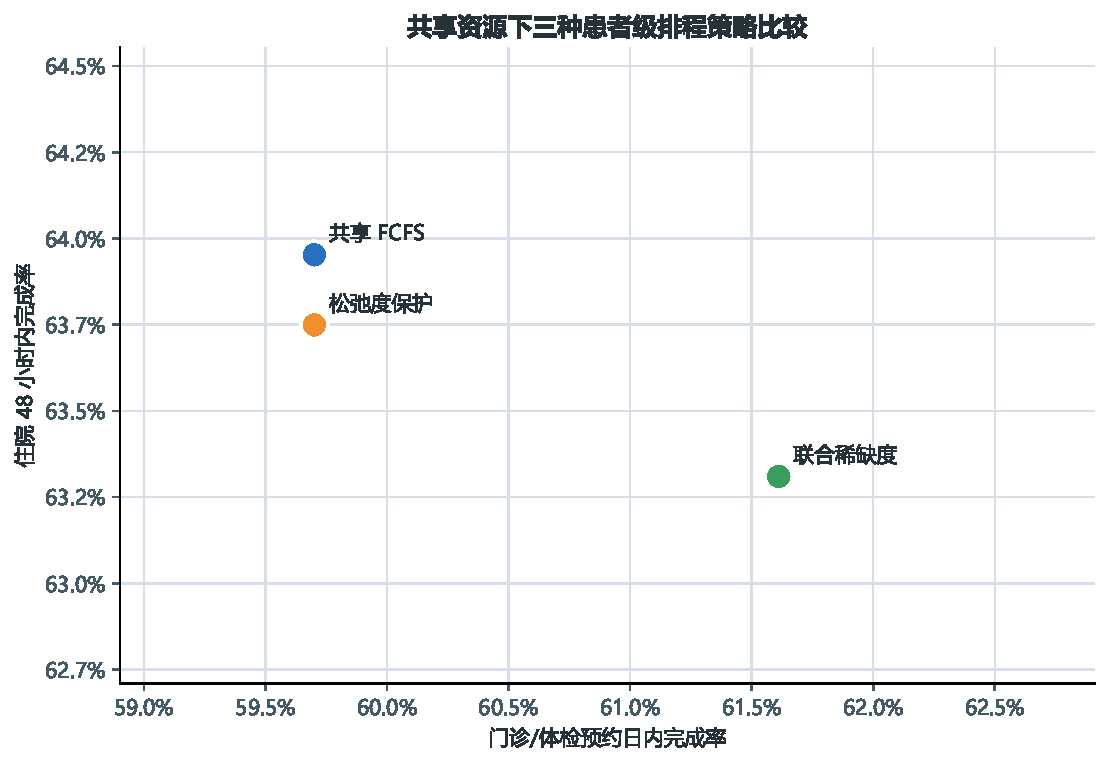
\includegraphics[width=0.58\textwidth]{fig04_policy_tradeoff.pdf}
  \caption{共享资源下三种排程策略比较}
  \label{fig:policy}
\end{figure}

\newpage
共享FCFS成功排入45\,260个留出期住院事件，未分配25\,511个。成功者首检等待中位数4.50小时、P90为40.42小时、P95为45.58小时；多项目患者跨室率为19.96\%。它比松弛度保护多完成144个住院事件；相对联合稀缺度则多完成455个住院事件，但少完成1\,834个门诊/体检计划日事件。由于赛题把住院48小时率设为唯一考核指标，且共享FCFS的背景率就是本文定义的不劣基线，最终推荐资源可行FCFS；若医院把背景服务下限提高到61.61\%附近，则应切换到联合稀缺度帕累托方案，而不能声称一套策略同时改善所有指标。

表\ref{tab:recommendation}给出推荐清单的开头部分。完整清单逐事件给出患者序位、项目序位、项目族、开始与结束时刻、设备、准备标记、转运时间和兼容证据层，可直接转换为预约系统导入表。

\begin{table}[H]
  \centering
  \caption{留出期住院患者推荐排程样例}
  \label{tab:recommendation}
  \begin{tabularx}{\textwidth}{r l r X l l}
\toprule
序位 & 事件 & 项目序位 & 项目族 & 时段 & 设备 \\
\midrule
1 & IP2024-000259 & 1 & 腹部/胃肠 & 04-01 08:30--08:40 & 门16(65) \\
2 & IP2024-000261 & 1 & 浅表器官 & 04-01 08:30--08:40 & 妇门2(75) \\
3 & IP2024-000265 & 1 & 浅表器官 & 04-01 08:35--08:45 & 门9(47) \\
4 & IP2024-000268 & 1 & 血管 & 04-01 08:50--09:00 & 病2(71) \\
4 & IP2024-000268 & 2 & 血管 & 04-01 09:40--09:50 & 病2(71) \\
5 & IP2024-000267 & 1 & 浅表器官 & 04-01 09:00--09:10 & 病3(72) \\
6 & IP2024-000271 & 1 & 血管 & 04-01 09:00--09:10 & 门3(42) \\
6 & IP2024-000271 & 2 & 介入/定位 & 04-01 09:45--09:55 & 门3(42) \\
\bottomrule
\end{tabularx}

\end{table}

\subsection{问题三：三类患者联合排程}

\subsubsection{共享压力场景的构造}

门诊和体检数据没有预约时刻。为回答“在三类患者同时占用设备时，住院48小时率能达到多少”，本文把两类患者的历史报告日期作为回顾性计划日，构造必须在该日工作块内完成的背景任务。该场景使用患者项目组合和日期负荷，但剔除报告时分、历史机房与历史医生。因此，它反映的是“当日需求压力下的可排程度”，不是对历史派单的重放。

背景事件的基础释放时刻为历史开单时刻与计划日工作块起点的较晚者，截止为计划日工作块终点；空腹任务只能进入上午并在10时前结束。对憋尿任务，准备完成时刻取开单时刻加准备提前量，最终释放为该时刻与计划日工作块起点的较晚者；这允许已提前准备的门诊/体检患者在开班时进入排程，而不会一律延迟到9时。住院事件仍使用精确开单时刻、准备约束和48小时截止。连续日历覆盖2024年3月30日至2025年4月2日：边界前2日承接尚未逾期的在制任务，边界后2日只用于完成3月31日开单患者的48小时观察窗；评价仅统计2024年4月1日至2025年3月31日释放或计划的事件。

\subsubsection{背景服务下限与住院主目标}

题面要求在满足门诊、体检需求的前提下最大化住院48小时率，但未给出背景服务的数值阈值。若直接把背景完成数放在住院指标之前，会在背景多排少量患者时牺牲题面唯一考核指标；若完全忽略背景，又不符合业务前提。因此本文以共享FCFS得到的背景计划日完成数$B_0$作为“不比基线差”的可审计下限：
\begin{equation}
  Z_B=\sum_{e\in\Ecal_O\cup\Ecal_P}y_e\geq B_0.
\end{equation}
在满足该下限的候选策略中，首先最大化住院48小时完成数
\begin{equation}
  \max Z_I=\sum_{e\in\Ecal_I}y_e.
\end{equation}
随后才比较背景增量、住院等待、跨室和设备负荷差。共享FCFS和联合稀缺度均满足$Z_B\geq B_0$，前者住院指标更高，故作为主推荐；后者背景服务率更高，作为医院提高背景下限时的帕累托备选。若医院能给出正式门诊/体检服务水平或急诊等级，应以该阈值和急诊硬保护替代$B_0$，不能长期把历史基线当成临床制度。

主策略先按计划日与释放时刻安排背景患者，再按住院释放时刻（由于截止均为开单后48小时，亦等价于最早截止顺序）进入共享日历；每个患者内部仍采用能力稀缺优先、同室优先和最早可行时隙搜索。因此“FCFS”只描述患者间主序，不等于忽略设备能力的简单排队。联合稀缺度备选则先按空腹标记、项目最小可用设备数和工作量安排背景任务，再按住院松弛度排入余量。两种过程都只初始化一次房间占用和医生负荷状态。

\subsubsection{联合排程结果}

主情景中，主推荐策略在留出期完成57\,341个背景事件，计划日完成率59.70\%；其中门诊完成42\,871个，体检完成14\,470个。住院完成45\,260个，48小时率63.95\%。联合稀缺度备选完成59\,175个背景事件，背景率61.61\%，但住院只完成44\,805个、住院率63.31\%。两个比例的分母均包含未分配事件，未因无可行设备或搜索失败而删除。

图\ref{fig:daily}给出14日滚动完成率；14日只用于压低日级随机波动、辨认趋势，不进入排程规则。住院率大部分时间在60\%--75\%之间，门诊/体检在2024年秋季出现明显下降、2025年初回升，与体检团检波动和背景总负荷一致。年度平均值不能替代日级监控；实际部署时应同时查看完成率、未来48小时已知需求和稀缺项目分钟数，再决定是否调班。

\begin{figure}[H]
  \centering
  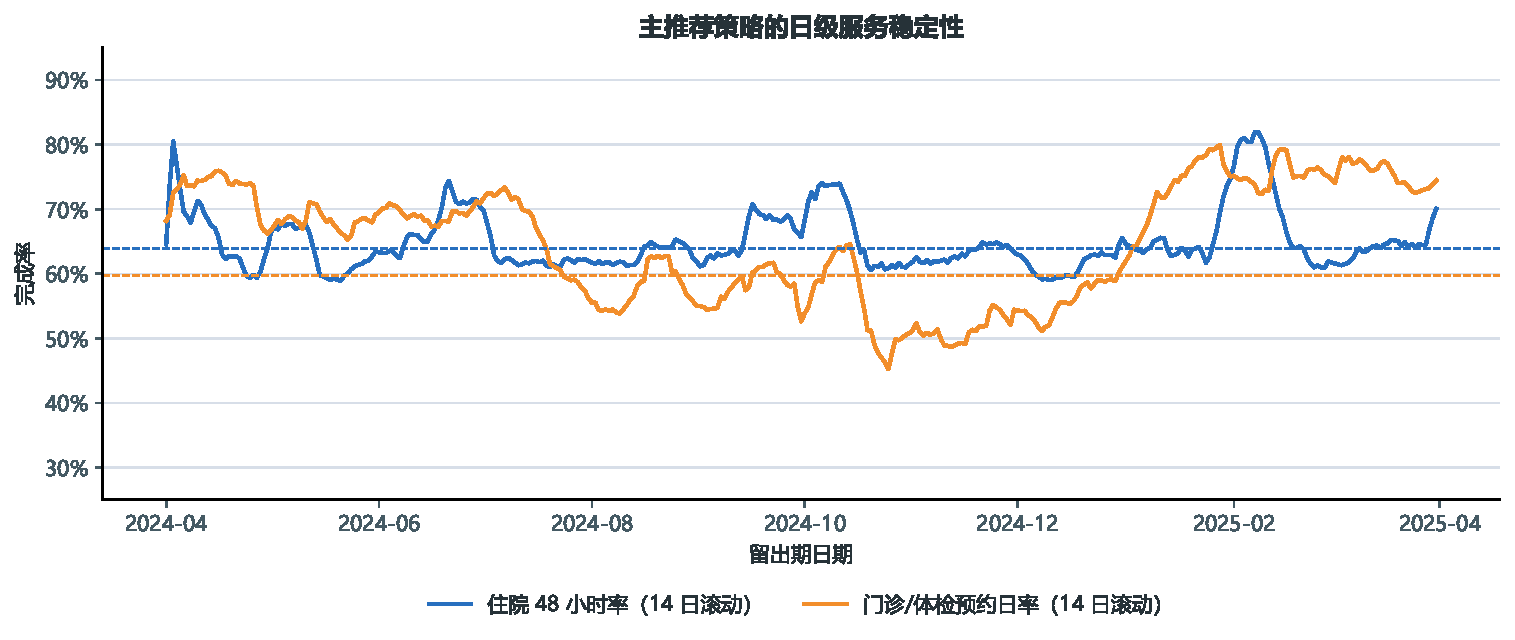
\includegraphics[width=\textwidth]{fig06_daily_performance.pdf}
  \caption{主推荐策略的日级服务稳定性}
  \label{fig:daily}
\end{figure}

图\ref{fig:gantt}展示主推荐策略留出期工作量最高的2024年10月14日。排程在12--13时保持午休断点，三类患者在各机房交错安排；床边B超主要服务住院患者，产科和门诊机房在上午承接体检与门诊，下午逐步释放给住院任务。图中每个色块均来自一条实际患者项目记录，不是总容量示意。

\begin{figure}[H]
  \centering
  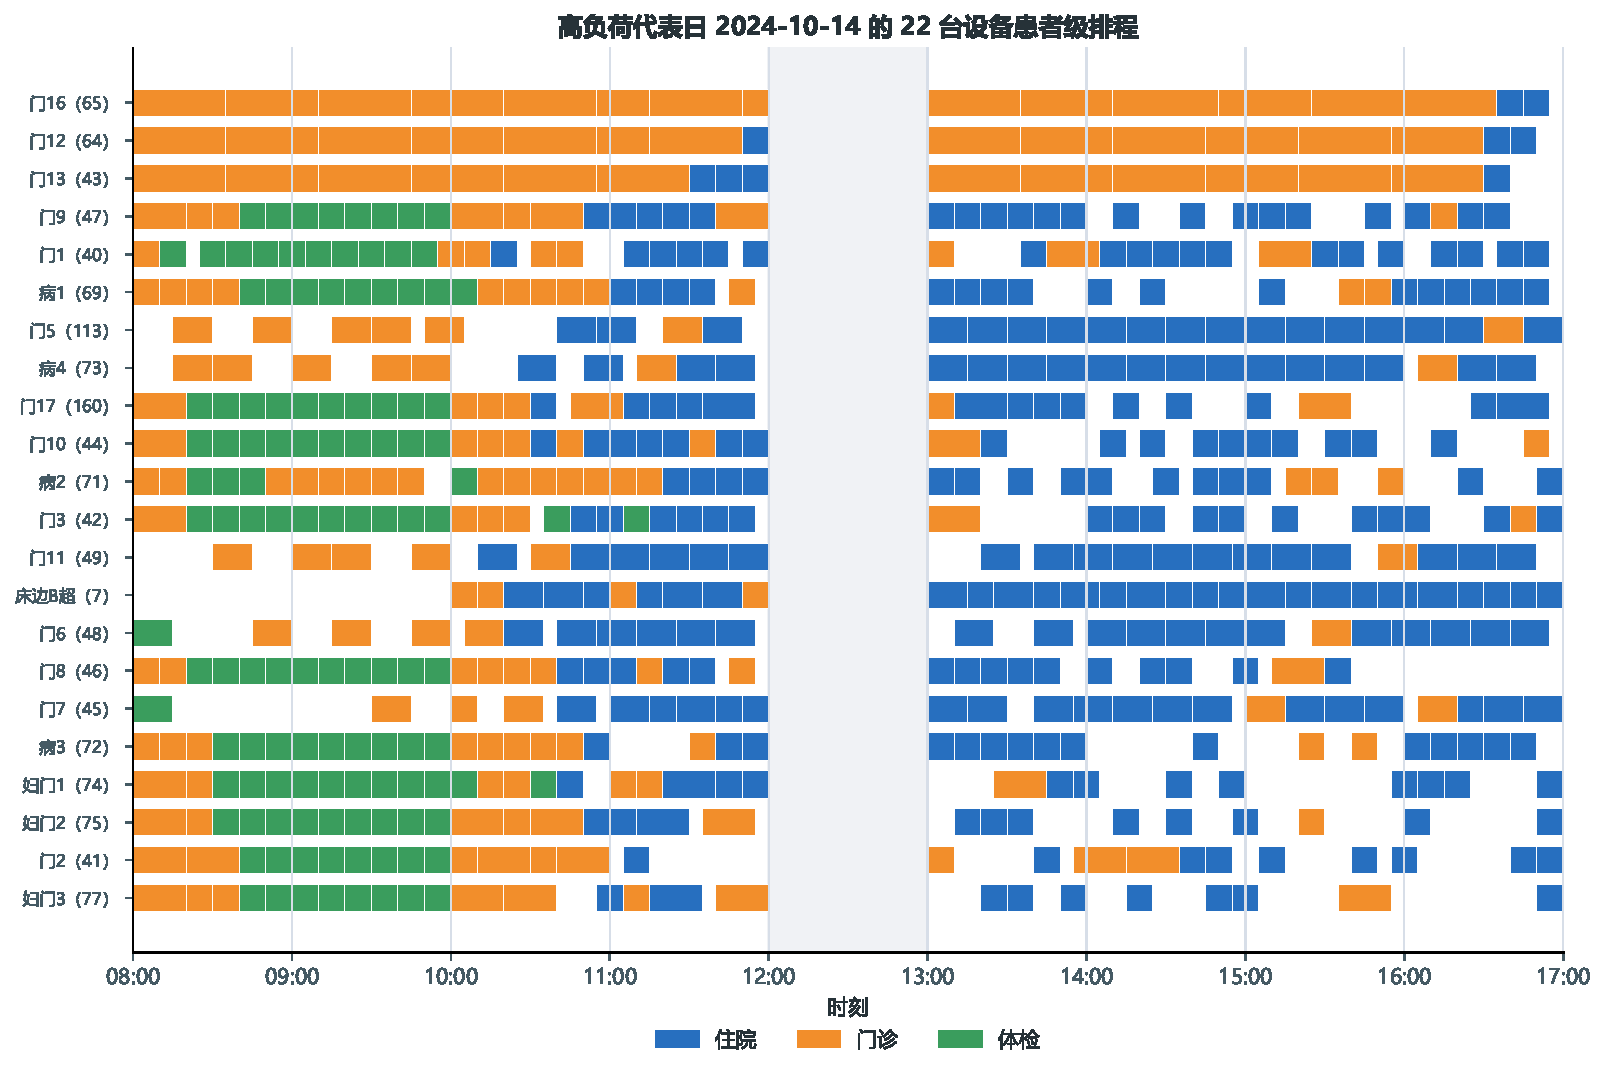
\includegraphics[width=\textwidth]{fig07_representative_gantt.pdf}
  \caption{高负荷代表日的22台设备患者级排程}
  \label{fig:gantt}
\end{figure}

设备日均占用率见图\ref{fig:utilization}. 7号床边B超达到73.95\%，显著高于其他设备的36.16\%--57.05\%，与表\ref{tab:capability}的唯一床旁能力一致。其余普通设备存在一定负荷差异；产科III/IV级设备占用相对较低并不表示可以撤销，因为它们承担的是不可替代的专项能力。

\begin{figure}[H]
  \centering
  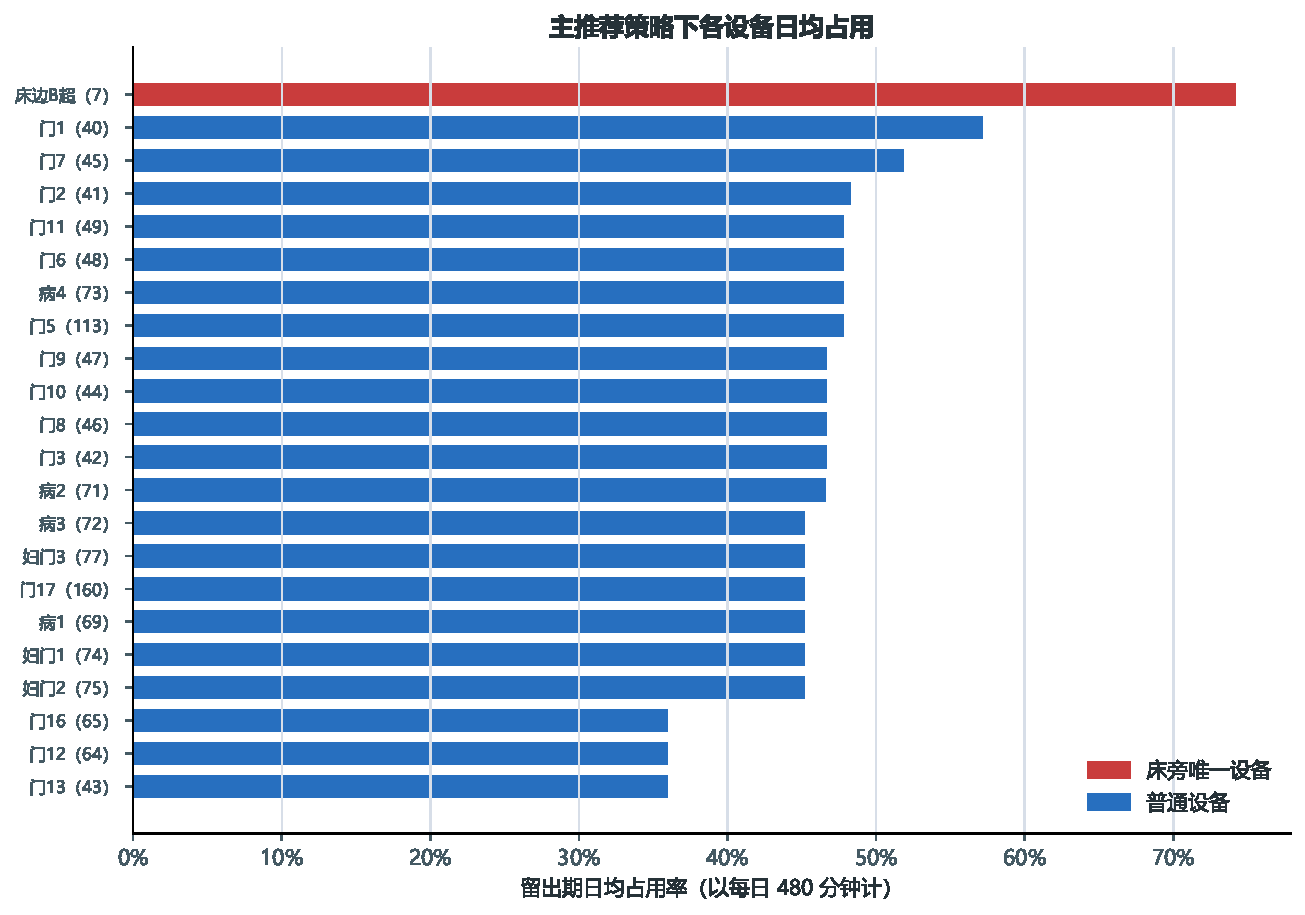
\includegraphics[width=0.88\textwidth]{fig08_room_utilization.pdf}
  \caption{主推荐策略下各设备日均占用率}
  \label{fig:utilization}
\end{figure}

\subsubsection{联合方案的实施建议}

由结果得到四项实施建议。

\begin{enumerate}
  \item 每次发布下一轮计划前，用未来48小时已知门诊、体检计划和住院在制队列重新构造滚动日历；已确认预约作为冻结层，新增住院患者只在余量中插入。
  \item 7号床边B超按未来48小时床旁任务上界分钟保护容量；当剩余容量已不能覆盖床旁需求或最紧迫床旁事件时，停止非床旁回填，并由医院决定是否启用具备床旁能力的备用设备或移动班次。
  \item 对64、43、65号产科高等级设备和45、44号儿科设备保留能力池，不以短期占用率为唯一裁撤依据；灵活项目优先落到能力覆盖广的普通设备。
  \item 若预计医生并发达到$c_{wt}$，优先调整医生班次而不是继续开放空机房。新增设备只有与相应医生资质和班次同时增加，才能转化为完成率。
\end{enumerate}

\section{模型的检验}

\subsection{独立可行性核验}

为避免调度器用自身逻辑证明自身正确，另写独立核验程序，只读取统一输入、最终排程和结果表，重新计算任务时长、占用区间和医生并发。核验对象为151\,020条项目任务、102\,986个已排事件。检查组见表\ref{tab:verification}，所有违规数均为0；最大观测医生并发为20，等于主容量最大值而未超出。

\begin{table}[H]
  \centering
  \caption{最终联合排程的独立核验结果}
  \label{tab:verification}
  \begin{tabularx}{\textwidth}{X r l}
\toprule
核验项目 & 违规数 & 结论 \\
\midrule
任务键、输入对应、时长 & 0 & 通过 \\
设备兼容、床旁位置 & 0 & 通过 \\
释放、截止、工作时段 & 0 & 通过 \\
房间、患者、转运冲突 & 0 & 通过 \\
医生并发容量 & 0 & 通过 \\
结果表聚合一致性 & 0 & 通过 \\
\bottomrule
\end{tabularx}

\end{table}

除表中项目外，还检查了5分钟网格、项目序位连续、空腹10时前完成、床旁7号机和输出聚合标记。所有成功事件的项目数均等于输入服务项目数；所有未成功事件在结果表中保留失败原因“截止前无完整可行方案”。因此63.95\%不是项目级完成比例，也不是删除未排患者后的条件比例。

\subsection{补充敏感性情景}

赛题明确要求考虑峰/平配置和约5\%复杂病例；二者已进入主模型。为审核数据证据与假设边界，本文另设置七个\textbf{补充检验}，它们不是赛题指定情景：取消5\%时长上浮、医生容量采用训练日下四分位、只允许严格项目级设备证据、憋尿准备45/90分钟、跨室转运5/15分钟。每次只改变一个因素，结果见表\ref{tab:sensitivity}和图\ref{fig:sensitivity}。

\begin{table}[H]
  \centering
  \caption{主推荐策略的补充敏感性检验}
  \label{tab:sensitivity}
  \begin{tabular}{lrrrr}
\toprule
情景 & 住院48h率 & 背景预约日率 & 条件等待P90/h & 排入分钟 \\
\midrule
主情景：5\%上界时长 & 63.95\% & 59.70\% & 40.42 & 1,819,800 \\
无特殊时长上浮 & 63.97\% & 59.70\% & 40.42 & 1,819,660 \\
医生容量下四分位 & 61.96\% & 58.95\% & 42.00 & 1,769,275 \\
仅严格设备兼容 & 71.57\% & 49.67\% & 45.33 & 1,664,965 \\
憋尿准备45分钟 & 63.89\% & 59.88\% & 40.25 & 1,821,400 \\
憋尿准备90分钟 & 64.12\% & 59.17\% & 40.17 & 1,815,485 \\
跨室转运5分钟 & 63.93\% & 59.71\% & 40.50 & 1,821,800 \\
跨室转运15分钟 & 63.99\% & 59.76\% & 40.33 & 1,819,020 \\
\bottomrule
\end{tabular}

\end{table}

\begin{figure}[H]
  \centering
  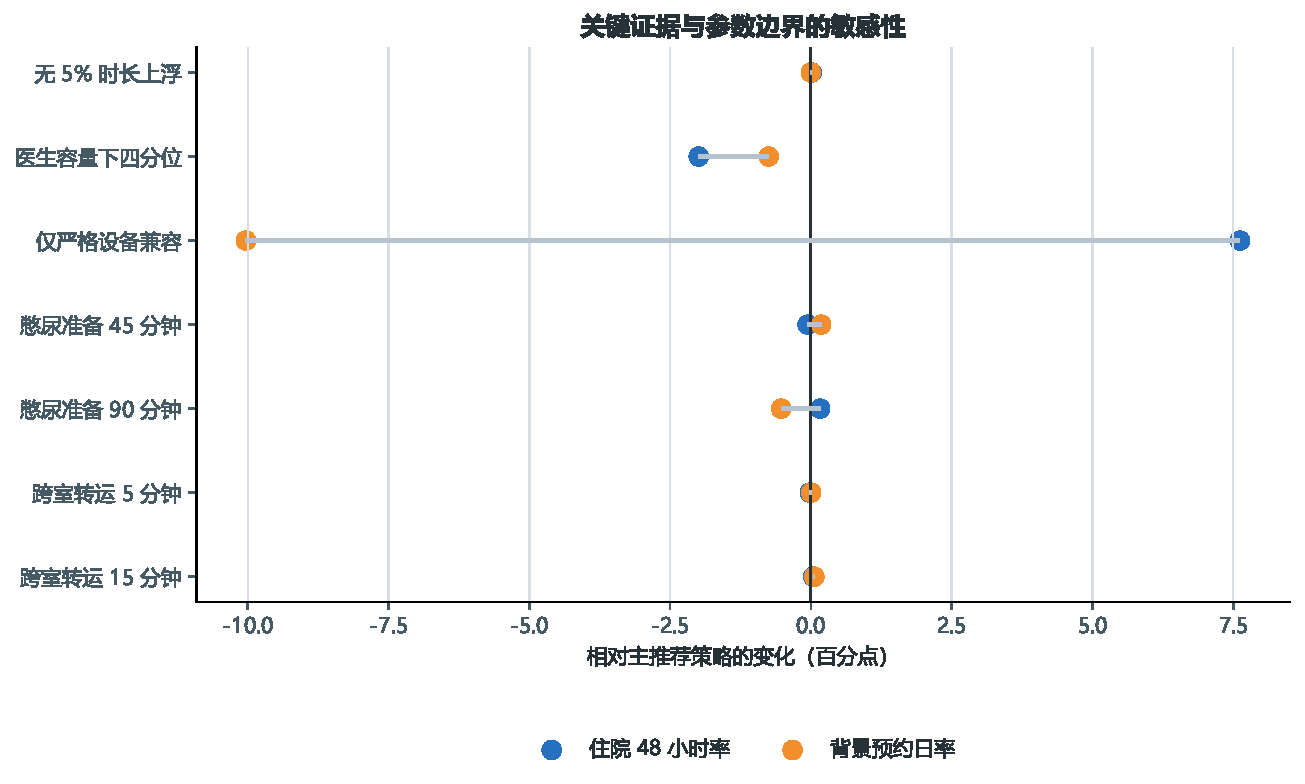
\includegraphics[width=0.70\textwidth]{fig05_sensitivity.pdf}
  \caption{补充证据与参数边界相对主情景的变化}
  \label{fig:sensitivity}
\end{figure}

取消特殊时长上浮后住院率只增加0.013个百分点，背景率几乎不变。原因是多数项目上界与名义值在5分钟离散后差异有限，且系统瓶颈主要来自项目兼容和峰值到达。该结果不否定赛题的5\%条件，而是说明其在当前时长分档下边际影响较小。

医生容量降至下四分位后，住院率由63.95\%降至61.96\%，背景率由59.70\%降至58.95\%，住院首检等待中位数由4.50小时升至8.08小时，表明住院48小时目标对医生班次明显敏感。相比之下，单纯增加普通设备若没有医生同步到位，改善有限。

只允许严格设备证据时，背景率降至49.67\%，住院率反升至71.57\%。这不是模型变好，而是大量体检和门诊项目因缺少严格项目级匹配被直接判为不可排，释放了容量给住院。该现象说明项目能力覆盖必须用两类指标联合解释；部署前应由超声科逐条确认50个回退项目的可用设备，确认后再冻结正式能力矩阵。

憋尿准备45分钟时住院率为63.89\%，90分钟时为64.12\%，背景率分别为59.88\%和59.17\%。准备更晚会使部分背景事件无法在计划日完成，却为住院释放少量容量；准备更早又会改变排序与碎片。因此准备时长不是单调优化旋钮，应由预约通知、到院时间和实际准备状态共同决定。

跨室转运5、10和15分钟时，住院率分别为63.93\%、63.95\%和63.99\%，背景率分别为59.71\%、59.70\%和59.76\%。完成率在三点上变化较小但非单调，这是离散时隙、候选顺序和局部容量碎片共同作用的结果，不表示更慢转运能提升临床效率。上线时应用实测诊室动线替代该参数。

\subsection{结构合理性分析}

本文结果与诊断资源调度文献中的两个结论一致：一是混合患者资源应把事前容量保护与动态优先级结合\cite{green2006,patrick2007}；二是超声预约应同时考虑检查室分配和随机时长，而不是只给患者时间不给房间\cite{chen2022}。不同之处在于，本文没有用仿真分布代替题目缺失字段，而是以题给区间构造可解释上下界，并把项目能力证据强弱直接放入敏感性。

\section{模型的评价}

\subsection{模型优点}

\begin{enumerate}
  \item \textbf{口径完整。} 事件、项目、设备和医生均有明确单位；未分配患者保留在分母，避免把项目完成率冒充患者完成率。
  \item \textbf{约束统一。} 问题二和问题三共用同一房间、医生、患者、兼容、准备和转运规则，主模型与回放模型不存在可行域差异。
  \item \textbf{证据可追溯。} 设备严格匹配、床旁明确和类别回退分别记录；训练期与留出期物理隔离，未来报告时刻和历史派单不进入决策。
  \item \textbf{方案可执行。} 输出下沉到每位住院患者的项目次序、开始时刻和机房，并给出代表日完整甘特图，而非仅报告总容量或理论上界。
  \item \textbf{权衡透明。} 联合策略同时报告两类服务率和等待分位数；严格兼容情景的住院虚增被识别为服务覆盖下降，而不是误写为性能提升。
\end{enumerate}

\subsection{模型局限}

第一，历史数据缺少真实预约时刻、扫查起止和报告提交时刻。本文用题给区间确定绝对时长，用最后项目结束代理报告完成，因此无法分离扫查与报告环节。第二，未来医生只有总并发容量，没有姓名、项目资质和班表；模型保证总人数不超限，但不能保证某一时刻恰有具备专项资质的医生。第三，门诊和体检只构造回顾性计划日压力，不能还原真实预约提前期、迟到、爽约和插队。第四，题面没有给出背景服务下限，本文只能以共享FCFS服务率构造不劣基线；若医院给出更高阈值，策略选择会沿帕累托前沿改变。第五，构造算法在给定策略族中求最早可行方案，未证明对全年大规模整数模型达到全局最优；本文的“最佳”只指三种已比较策略中住院主指标最高且背景不低于基线。

\section{模型的改进与推广}

\subsection{数据与求解方法的改进}

若医院能够补充扫查开始、扫查结束、报告提交、预约时刻和医生项目资质，模型可作三项升级：其一，分别估计扫查时长和报告时长，以双阶段队列替代完成代理；其二，以医生—项目资质矩阵替代总并发容量，形成设备与医生双匹配；其三，用真实预约、迟到与爽约分布进行滚动随机优化，并把已确认预约冻结、未确认预约柔性调整。运行层面的刷新频率和冻结窗口应由叫号提前量、患者到院状态及系统响应时间标定，不在缺少现场数据时预设固定分钟数。

\subsection{医院内部推广与跨机构迁移}

模型的可推广部分是“事件—项目—双资源—时间窗”结构，而不是A医院的具体房号、日班时间或10分钟转运。在A医院内部，心电、CT、MRI等多资源检查可沿用患者完整性、能力兼容和截止期约束，但必须重新定义服务时长、准备要求和人员资质。迁移到其他医院时，应先以当地设备清单、班表和患者动线替换配置参数，再用本地时间顺序留出期评价；不应直接移植本文的63.95\%结果。

部署可采用“计划层—执行层—反馈层”闭环。计划层每日生成未来48小时容量保护；执行层读取到院、准备完成、急诊插入和设备停机状态；反馈层按日监控两类完成率、未排原因、等待分位数和改号次数。只有在前瞻试点中同时保持门诊/体检服务和住院48小时指标，才将新策略固化为正式规则。

\subsection{主要结论}

本文完成了超声预约问题的患者级联合建模。问题一得到训练期科室需求、11类项目时长、22台设备能力证据和星期—5分钟医生容量；床旁7号机是最明确的单点瓶颈。问题二在完整共享资源约束下输出住院患者项目顺序、时段和机房；问题三把门诊、体检与住院置于同一连续年度日历。以共享FCFS背景率为不劣基线时，资源可行FCFS在留出期取得住院63.95\%、背景59.70\%的完成率，是三个候选策略中住院主指标最高者；联合稀缺度以住院率降至63.31\%为代价把背景率提高到61.61\%，构成另一帕累托点。独立核验未发现约束违规，但医生容量和设备项目证据对结果影响明显。因而实施路线不是单纯增加设备，而是先确认正式背景服务阈值和项目能力清单、保护床旁与专项设备、保障高峰医生并发，再沿可接受的服务权衡选择患者级滚动排程策略。

\label{body:lastpage}

\clearpage
\section{参考文献}
\begingroup
\renewcommand{\refname}{参考文献}
\zihao{-4}\songti
\setlength{\itemsep}{3pt}
\begin{thebibliography}{99}

\bibitem{gupta2008}
GUPTA D, DENTON B. Appointment scheduling in health care: Challenges and opportunities[J]. IIE Transactions, 2008, 40(9): 800--819. DOI: \url{https://doi.org/10.1080/07408170802165880}.

\bibitem{ahmadi2017}
AHMADI-JAVID A, JALALI Z, KLASSEN K J. Outpatient appointment systems in healthcare: A review of optimization studies[J]. European Journal of Operational Research, 2017, 258(1): 3--34. DOI: \url{https://doi.org/10.1016/j.ejor.2016.06.064}.

\bibitem{nhc2020}
国家卫生健康委员会办公厅. 关于进一步完善预约诊疗制度加强智慧医院建设的通知：国卫办医函〔2020〕405号[EB/OL]. (2020-05-21)[2026-08-24]. \url{https://www.nhc.gov.cn/yzygj/c100068/202005/43b2d23ff48448ffae96700bc6eaccd7.shtml}.

\bibitem{chenjuan2023}
陈娟, 李志会, 赵浩, 等. 分时段分项目组多途径预约模式在妇幼专科医院超声检查中的应用[J]. 中国妇幼卫生杂志, 2023, 14(6): 77--80. DOI: \url{https://doi.org/10.19757/j.cnki.issn1674-7763.2023.06.014}.

\bibitem{marynissen2019}
MARYNISSEN J, DEMEULEMEESTER E. Literature review on multi-appointment scheduling problems in hospitals[J]. European Journal of Operational Research, 2019, 272(2): 407--419. DOI: \url{https://doi.org/10.1016/j.ejor.2018.03.001}.

\bibitem{apergi2020}
APERGI L A, BARAS J S, GOLDEN B L, et al. An optimization model for multi-appointment scheduling in an outpatient cardiology setting[J]. Operations Research for Health Care, 2020, 26: 100267. DOI: \url{https://doi.org/10.1016/j.orhc.2020.100267}.

\bibitem{wang2019}
王珊珊, 李金林, 彭春, 等. 不确定服务时间下分布式鲁棒门诊预约调度和排程[J]. 系统工程学报, 2019, 34(4): 566--576.

\bibitem{hrhospital2025}
华容区人民医院. 超声科流程及注意事项[EB/OL]. (2025-08-20)[2026-08-24]. \url{https://www.hbhr.gov.cn/hrqxxgk/xxgkml/ggqsydwxxgk/wsjk/hrqrmyy/202508/t20250821_720866.html}.

\bibitem{zhu2015}
朱顺痣, 王大寒, 何亚男, 等. 基于时间序列模型的医院门诊量分析与预测[J]. 中国科学技术大学学报, 2015, 45(10): 795--803. DOI: \url{https://doi.org/10.3969/j.issn.0253-2778.2015.10.001}.

\bibitem{xiang2009}
向前, 陈平雁. 预测医院门诊量的ARIMA模型构建及应用[J]. 南方医科大学学报, 2009, 29(5): 1076--1078. PMID: 19460744.

\bibitem{luo2017}
LUO L, LUO L, ZHANG X, et al. Hospital daily outpatient visits forecasting using a combinatorial model based on ARIMA and SES models[J]. BMC Health Services Research, 2017, 17: 469. DOI: \url{https://doi.org/10.1186/s12913-017-2407-9}.

\bibitem{lai2025}
LAI C H, LU Y J, CHEN P S. Using data-driven techniques to predict outpatient ultrasound examination time for the multi-clinic outpatient appointment scheduling problem[J]. Communications in Statistics-Simulation and Computation, 2025, 54(9): 3358--3376. DOI: \url{https://doi.org/10.1080/03610918.2024.2349168}.

\bibitem{patrick2008}
PATRICK J, PUTERMAN M L, QUEYRANNE M. Dynamic multipriority patient scheduling for a diagnostic resource[J]. Operations Research, 2008, 56(6): 1507--1525. DOI: \url{https://doi.org/10.1287/opre.1080.0590}.

\bibitem{patrick2007}
PATRICK J, PUTERMAN M L. Improving resource utilization for diagnostic services through flexible inpatient scheduling: A method for improving resource utilization[J]. Journal of the Operational Research Society, 2007, 58(2): 235--245. DOI: \url{https://doi.org/10.1057/palgrave.jors.2602242}.

\bibitem{chen2022}
CHEN P S, CHEN G Y H, LIU L W, et al. Using simulation optimization to solve patient appointment scheduling and examination room assignment problems for patients undergoing ultrasound examination[J]. Healthcare, 2022, 10(1): 164. DOI: \url{https://doi.org/10.3390/healthcare10010164}.

\bibitem{qiao2024}
乔岩, 冉伦, 李金林, 等. 基于两阶段随机规划的远程会诊预约调度问题研究[J]. 中国管理科学, 2024, 32(1): 86--93. DOI: \url{https://doi.org/10.16381/j.cnki.issn1003-207x.2020.1989}.

\bibitem{nhc2022}
国家卫生健康委员会办公厅. 关于印发超声诊断等5个专业医疗质量控制指标（2022年版）的通知：国卫办医函〔2022〕161号[EB/OL]. (2022-05-27)[2026-08-24]. \url{https://www.nhc.gov.cn/yzygj/c100068/202205/164e6556f6d34c33a3344fec9a2c5074.shtml}.

\end{thebibliography}
\endgroup


\clearpage
\appendix
\section{支撑材料文件说明}

计算所用程序和结果数据保存在\path{supporting_materials}目录。限于篇幅，本附录选录与各模型直接对应的核心算法，主要文件见表\ref{tab:appendix-files}。

\begin{table}[H]
\centering
\caption{主要程序及功能}
\label{tab:appendix-files}
\begin{tabularx}{\textwidth}{p{0.43\textwidth}X}
\toprule
文件 & 功能 \\
\midrule
\path{code/analyze_p1.py} & 构造申请事件，分析需求、项目工时、科室结构与医生容量 \\
\path{code/build_unified_inputs.py} & 生成统一事件表、项目表和项目设备兼容集合 \\
\path{code/run_unified_scheduler.py} & 患者级可行性内核及问题二纯住院调度 \\
\path{code/run_pre_freeze_scenarios.py} & 问题二候选策略与问题三背景下限扫描 \\
\path{code/benchmark_exact_scheduler.py} & 问题二CP-SAT精确子问题对照 \\
\path{code/benchmark_exact_p3_scheduler.py} & 问题三联合调度CP-SAT精确子问题对照 \\
\path{code/verify_unified_schedule.py} & 从导出排程独立重建并检查全部约束 \\
\path{results/p1/} & 问题一需求、工时、峰平阈值与预测检验结果 \\
\path{results/final_frozen/} & 问题二、问题三及敏感性结果的机器可读文件 \\
\bottomrule
\end{tabularx}
\end{table}

计算顺序与正文一致：先完成数据预处理和问题一分析，再构建统一调度输入并求解问题二、三，随后计算精确子问题、校准和敏感性情景，最后独立检验排程可行性。各程序从题目原始附件或上一步结果读取数据，完整字段说明保存在同目录说明文档中。

\section{数据预处理程序}

数据预处理先由\path{analyze_p1.py}中的\path{expand_embedded_project_lists}按源系统明确的\path{][}边界拆分项目，再由\path{build_unified_inputs.py}中的\path{load_source}按“来源、患者编号、精确开单时刻”聚合事件、删除精确重复明细并生成稳定事件编号。下面直接摘录实际源码；函数后续的项目表字段整理保留在完整文件中。

\lstinputlisting[style=paperpython,firstline=218,lastline=238,firstnumber=218,caption={显式复合项目拆分的实际源码}]{../supporting_materials/code/analyze_p1.py}

\lstinputlisting[style=paperpython,firstline=141,lastline=177,firstnumber=141,caption={事件聚合与去重的实际源码}]{../supporting_materials/code/build_unified_inputs.py}

\lstinputlisting[style=paperpython,firstline=179,lastline=201,firstnumber=179,caption={模拟边界与稳定事件编号的实际源码}]{../supporting_materials/code/build_unified_inputs.py}

\section{问题一程序}

问题一按来源构造完整日序列，严格以2024年4月1日为时间分界，在训练期估计候选预测器并在留出期计算误差。对数岭回归由线性方程直接求解，峰平阈值只读取训练子集。以下均为\path{analyze_p1.py}的实际代码。

\lstinputlisting[style=paperpython,firstline=533,lastline=590,firstnumber=533,caption={时间留出预测与误差计算的实际源码}]{../supporting_materials/code/analyze_p1.py}

\lstinputlisting[style=paperpython,firstline=593,lastline=615,firstnumber=593,caption={训练期峰平分位数的实际源码}]{../supporting_materials/code/analyze_p1.py}

\section{问题二程序}

问题二由\path{task_order_candidates}生成四类项目顺序，\path{tentative_plan}逐项预留日历；任一任务失败时逆序释放此前位置，全部成功时保留预留结果。\path{plan_event}先尝试共同设备，再放开跨室安排。下面直接摘录\path{run_unified_scheduler.py}中的实现。

\lstinputlisting[style=paperpython,firstline=484,lastline=531,firstnumber=484,caption={候选项目序列与失败回滚的实际源码}]{../supporting_materials/code/run_unified_scheduler.py}

\lstinputlisting[style=paperpython,firstline=534,lastline=559,firstnumber=534,caption={共同设备优先的患者级排程实际源码}]{../supporting_materials/code/run_unified_scheduler.py}

\section{问题三程序}

问题三的正式下限按全评价期背景事件总数计算。\path{build_p3_candidate}先生成住院优先基线；若其未达到下限，则从空日历执行\path{global_deficit_repair}分支，先排至全期背景目标，再排住院和剩余背景。\path{solve_p3_epsilon}仅从达到下限的候选中按住院完成数及等待指标选择。下面直接摘录\path{run_pre_freeze_scenarios.py}中的两个实际函数。

\lstinputlisting[style=paperpython,firstline=216,lastline=293,firstnumber=216,caption={住院基线与全局缺口重构分支的实际源码}]{../supporting_materials/code/run_pre_freeze_scenarios.py}

\lstinputlisting[style=paperpython,firstline=305,lastline=357,firstnumber=305,caption={全期背景下限与候选选择的实际源码}]{../supporting_materials/code/run_pre_freeze_scenarios.py}

\section{模型验证程序}

验证程序从导出的任务表重新建立区间和容量占用，不调用主调度器的插入函数。除逐任务检查释放、截止、准备和设备能力外，还独立检查设备与患者区间重叠、跨室转运以及每个5分钟槽的医生并发。下面直接摘录\path{verify_unified_schedule.py}中的互斥与容量复核；问题二、三精确子问题分别见两个CP-SAT程序。

\lstinputlisting[style=paperpython,basicstyle=\ttfamily\fontsize{8.5pt}{9.5pt}\selectfont,firstline=220,lastline=364,firstnumber=220,caption={互斥、转运与医生容量复核的实际源码}]{../supporting_materials/code/verify_unified_schedule.py}


\end{document}
